%\documentclass[14pt]{article}
%\renewcommand{\baselinestretch}{1.5}
\documentclass[14pt,a4paper]{PhDthesis}
\usepackage[utf8]{inputenc}
\usepackage[russian]{babel}
\usepackage{amsmath}
\usepackage{amssymb}
\usepackage{fullpage}
\usepackage{indentfirst}
\usepackage{graphicx}
\usepackage{tabularx,multirow}
\usepackage{psfrag}
\usepackage{cite}

\usepackage{listings}
\usepackage{ucs}
\usepackage{listings}
\usepackage{amsmath}
\usepackage{tabularx}
\usepackage{hyperref}
\usepackage{tikz}
\usetikzlibrary{positioning,arrows}
\usepackage{graphicx}
\textwidth=16cm
\usepackage{amssymb}
\usepackage{fullpage}
\usepackage{indentfirst}
\usepackage{graphicx}
\usepackage{psfrag}
\usepackage{cite}
\usepackage{fullpage}
%\usepackage[dvips]{graphicx}
%\graphicspath{{images/}}
\lstset{inputencoding=utf8x, extendedchars=\true, captionpos=b, tabsize=3, keywordstyle=\color{blue},commentstyle=\color{green}, stringstyle=\color{red}, showstringspaces=false, basicstyle=\footnotesize,emph={label}, texcl}
%\lstset{texcl}
%\lstset{extendedchars=\true}
\lstset{
literate={а}{{\selectfont\char224}}1
{б}{{\selectfont\char225}}1
{в}{{\selectfont\char226}}1
{г}{{\selectfont\char227}}1
{д}{{\selectfont\char228}}1
{е}{{\selectfont\char229}}1
{ё}{{\"e}}1
{ж}{{\selectfont\char230}}1
{з}{{\selectfont\char231}}1
{и}{{\selectfont\char232}}1
{й}{{\selectfont\char233}}1
{к}{{\selectfont\char234}}1
{л}{{\selectfont\char235}}1
{м}{{\selectfont\char236}}1
{н}{{\selectfont\char237}}1
{о}{{\selectfont\char238}}1
{п}{{\selectfont\char239}}1
{р}{{\selectfont\char240}}1
{с}{{\selectfont\char241}}1
{т}{{\selectfont\char242}}1
{у}{{\selectfont\char243}}1
{ф}{{\selectfont\char244}}1
{х}{{\selectfont\char245}}1
{ц}{{\selectfont\char246}}1
{ч}{{\selectfont\char247}}1
{ш}{{\selectfont\char248}}1
{щ}{{\selectfont\char249}}1
{ъ}{{\selectfont\char250}}1
{ы}{{\selectfont\char251}}1
{ь}{{\selectfont\char252}}1
{э}{{\selectfont\char253}}1
{ю}{{\selectfont\char254}}1
{я}{{\selectfont\char255}}1
{А}{{\selectfont\char192}}1
{Б}{{\selectfont\char193}}1
{В}{{\selectfont\char194}}1
{Г}{{\selectfont\char195}}1
{Д}{{\selectfont\char196}}1
{Е}{{\selectfont\char197}}1
{Ё}{{\"E}}1
{Ж}{{\selectfont\char198}}1
{З}{{\selectfont\char199}}1
{И}{{\selectfont\char200}}1
{Й}{{\selectfont\char201}}1
{К}{{\selectfont\char202}}1
{Л}{{\selectfont\char203}}1
{М}{{\selectfont\char204}}1
{Н}{{\selectfont\char205}}1
{О}{{\selectfont\char206}}1
{П}{{\selectfont\char207}}1
{Р}{{\selectfont\char208}}1
{С}{{\selectfont\char209}}1
{Т}{{\selectfont\char210}}1
{У}{{\selectfont\char211}}1
{Ф}{{\selectfont\char212}}1
{Х}{{\selectfont\char213}}1
{Ц}{{\selectfont\char214}}1
{Ч}{{\selectfont\char215}}1
{Ш}{{\selectfont\char216}}1
{Щ}{{\selectfont\char217}}1
{Ъ}{{\selectfont\char218}}1
{Ы}{{\selectfont\char219}}1
{Ь}{{\selectfont\char220}}1
{Э}{{\selectfont\char221}}1
{Ю}{{\selectfont\char222}}1
{Я}{{\selectfont\char223}}1
}


 
\begin{document}
\thispagestyle{empty}
\begin{center}
\enlargethispage{3cm}

{\Large\sc Министерство образования и науки Российской Федерации}

\bigskip
{\large Федеральное государственное бюджетное образовательное учреждение высшего профессионального образования}

{\large Алтайский государственный университет}

\bigskip
{\large Физико-технический факультет}

\bigskip
{Кафедра радиофизики и теоретической физики }
\bigskip

\vfill
\vfill
{\Large\sf\bf <<Физическая реализация квантовых вычислений на основе квантовых точек>>}
\bigskip

{\sf (Отчет по научно-исследовательской практике)}


\vfill
\hfill
\parbox[b]{7cm}{\raggedright
Выполнил\\
студент группы $511$м \\
{}\rule{0pt}{2ex}\hrulefill Донцов А.\,А.\\
Руководитель практики\\
к.ф.-м.н.\\
{}\rule{0pt}{2ex}\hrulefill Волков Н.\,В.\\
Отчет представлен на кафедру РТФ\\
{}<<\makebox[2em]{\rule{0pt}{4ex}\hrulefill}>>\hrulefill \ 2012\ г.\\
Оценка \hrulefill\\
Заведующий кафедрой РТФ\\
д.ф.-м.н., проф. \\
{}\rule{0pt}{2ex}\hrulefill Лагутин А.\,А.\\
}

\vfill
\vfill

\center
Барнаул --- 2012
\end{center}
\newpage
\tableofcontents
\newpage
\setcounter{chapter}{1}
\section*{Введение}
\addcontentsline{toc}{section}{Введение}
\textbf{\textit{Актуальность.}} В настоящее время сделана большая работа в области построения квантовых вычислительных машин, разработана большая теоретическая база. Хотя до сих пор полноценный квантовый компьютер не был построен, но уже сейчас реализованы некоторые прототипы квантового компьютера. При построении квантовых вычислительных машин возникают так же технологические трудности, например, такие как потеря когерентности. Отсутствие хороших средств для моделирования и разработки квантовых алгоритмов затрудняет работу по построению новых алгоритмов, что подтверждается наличием малого числа действительно квантовых алгоритмов \cite{Omer:2003, Vizzotto:2010}. Для реализации квантовых алгоритмов нужно выполнить следующие условия:
\begin{itemize}
  \item адекватно представлять квантовую информацию; 
 
  \item выполнять универсальный набор квантовых унитарных преобразований;

  \item приготавливать начальное состояние;
  
  \item измерять конечный результат.
\end{itemize}
Для реализации этих требований хорошо подходят квантовые точки – системы атомов, имеющие размер ∼1 нм (то есть $10^{-9}$ м). Электрон в квантовой точке локализован, поэтому энергетический спектр квантовой точки является дискретным, как
у атома, так что квантовые точки можно считать искусственными атомами. Дискретность электронных состояний в квантовой точке и наличие у электрона собственного вращательного момента (спина) могут быть использованы при конструировании логических элементов
(вентилей) \cite{kokin:2004ru}.

\textbf{\textit{Цель}.} Построение и описание математической модели квантовых вычислений, основанных на применении квантовых точек, основанных на полупроводниковых гетероструктурах.

Разработка математического представления квантовых вычислений и квантовой памяти.

\textbf{\textit{Задачи}.} Формулировка и решение задачи нахождения собственных значений (энергетического спектра) и собственных функций электрона,
представляющего собой квантовую точку.

Формулировка условий, при которых с помощью квантовой точки возможно проведение квантовых вычислений.

\section{Квантовая точка, квантовый гармонический осциллятор}

Квантовая точка --- это фрагмент проводника или полупроводника, содержащий в себе электрон или электроны, ограниченные со всех сторон каким-либо потенциальным барьером, в качестве барьера довольно часть применяют примеси каких-либо других веществ. Потенциал, создаваемый в квантовой точке,
ограничивает движение носителей заряда во всех трёх пространственных измерениях. Характерные размеры квантовой точки от 10 нм до 100 нм.

Квантовую точку можно рассматривать как потенциальную яму содержащую в себе частицу. Поведение такой частицы описывается уравнением гармонического осциллятора, при рассмотрении двумерного случая, гамильтониан такой системы имеет вид: 
\begin{equation}
H = \dfrac{p^{2}}{2m} + V(x),
\end{equation}
где $V(x) = 0$ при $0 < x < L$ и $V(x) = \infty$ в противном случае. Собственные состояние в координатном представлении имеют вид \ref{energi}
\begin{equation}
|\psi_{n}\rangle = \sqrt{\frac{2}{L}}\sin \Bigr(\frac{\pi x n}{L} \Bigr)
\end{equation}
и	
\begin{equation}
E_{n} = \frac{n^{2} \pi^{2}}{2 m L^{2}} \label{energi}.
\end{equation}
Таким образом гамильтониан принимает дискретные значения.
Рассморим двумерную потенциальную яму с бесконечными стенками и пусть в ней у частицы только два энергетических уровня. 
\begin{figure}[h!]
\centering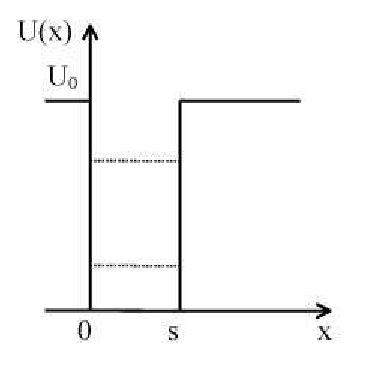
\includegraphics[width=.50\textwidth]{images/potents.eps}
\caption{Одномерная прямоугольная потенциальная яма, $U(x)$ - потенциальная энергия}\label{ris:potents}
\end{figure}
Тогда волновую функцию можно записать как $|\psi\rangle = a|\psi_{1}\rangle + b|\psi_{2}\rangle$. Поскольку
\begin{equation}
|\psi\rangle = e^{(E_{1} - E_{2})/2t} [a e^{-i \omega t}|\psi_{1}\rangle + b e^{i \omega t} |\psi_{2}\rangle],
\end{equation}
где $\omega = (E_{1} - E_{2})/2$, можно рассматривать только амплитуды $a$ и $b$, так что соостояние представляется абстрактным двухкомпонентным вектором
\begin{equation}
|\psi\rangle = \begin{bmatrix} \psi_{n} \\ \psi_{m} \end{bmatrix}.
\end{equation}
Таким образом, эта двухуровневая система представляет кубит. Его эволюция во времени описывается эффективным гамильтонианом $H = h \omega Z$ \cite{Vontsovskiy:1983ru, JaySau:2010}.

Предположим, что данная система подвергается внешнему воздействию электромагнитного поля, изменяющегося во времени по закону 
$\epsilon (t) = \epsilon _{0} e^{-t/|\tau|}$, и направленному вдоль оси $Oz$. 

Если внешнее возмущение удовлетворяет условию применимости теории возмущений, вероятность перехода может быть вычислена в рамках нестационарной теории возмущений. Амплитуда процесса в первом порядке теории возмущений имеет вид 
\begin{equation}
A_{mn} = \frac{1}{i \hbar} \int_{t}^{\tau} \langle f_{n}  |\hat{V}(\textbf{r}, t)|f_{m}\rangle e^{i \omega f_{mn} t} dt,
\end{equation}
где $\omega_{mn} = (E_{n} - E_{m})/\hbar$ --- частота перехода. С амплитудой простым соотношением связана вероятность перехода с уровня с энергией $E_{m}$ на уровень с энергией $E_{n}$
\begin{equation}
W_{mn} = | A_{mn}|^{2} = \frac{1}{i \hbar} \Bigl |\int_{t}^{\tau} \langle f_{n}  |\hat{V}(\textbf{r}, t)|f_{m}\rangle e^{i \omega f_{mn} t} dt \Bigr |^{2}.
\end{equation}

Введём повышающий и понижающий операторы $a^{+}$ и $a$,  соответственно определённые, как
\begin{equation}
a^{+} = \frac{1}{\sqrt{2m \hbar \omega}} (m \omega x + ip),
\end{equation}
\begin{equation}
a = \frac{1}{\sqrt{2m \hbar \omega}} (m \omega x - ip).
\end{equation}
Здесь $a^{+}|\psi\rangle$ является собственным состоянием гамильтониана $H$ с энергией $E + \hbar\omega$, $a|\psi\rangle$ собственное состояние с энергией  $E - \hbar\omega$ \cite{Nilsen:2001ru}.

Физически понижающий и повышающий операторы можно реализовать следующим образом: если на потенциальную яму с электроном действует магнитное поле, то в зависимости от направления магнитного поля и проекции спина электрона, электрон может переходить с уровня на уровень.

Кубиты можно представить энергетическими собственными состояниями $|n\rangle$
\begin{eqnarray}
|00\rangle_{L} \longleftrightarrow |0\rangle,   \\
|01\rangle_{L} \longleftrightarrow |1\rangle,\\
|10\rangle_{L} \longleftrightarrow \frac{|0\rangle + |1\rangle}{\sqrt{2}} \label{plus-position},\\
|10\rangle_{L} \longleftrightarrow \frac{|0\rangle - |1\rangle}{\sqrt{2}} \label{minus-position}.
\end{eqnarray}
Здесь индекс $L$ означает логические состояния, а не состояния осциллятора.
Пусть система эволюционирует в течении времени $t = \pi / \hbar\omega$, при этом собственные состояния преобразуются по закону
\begin{equation}
|n\rangle \rightarrow \exp(-i\pi a^{+} a)|n\rangle = (-1)^{n}|n\rangle.
\end{equation}
Состояние $|0\rangle$ остаётся неизменным, $|1\rangle$ меняет свой знак.
Состояние (\ref{plus-position}) и (\ref{minus-position}) изображены на сфере Блоха (см.рис.~\ref{ris:image1}).

\begin{figure}[h]
\begin{minipage}[h]{0.49\linewidth}
\center{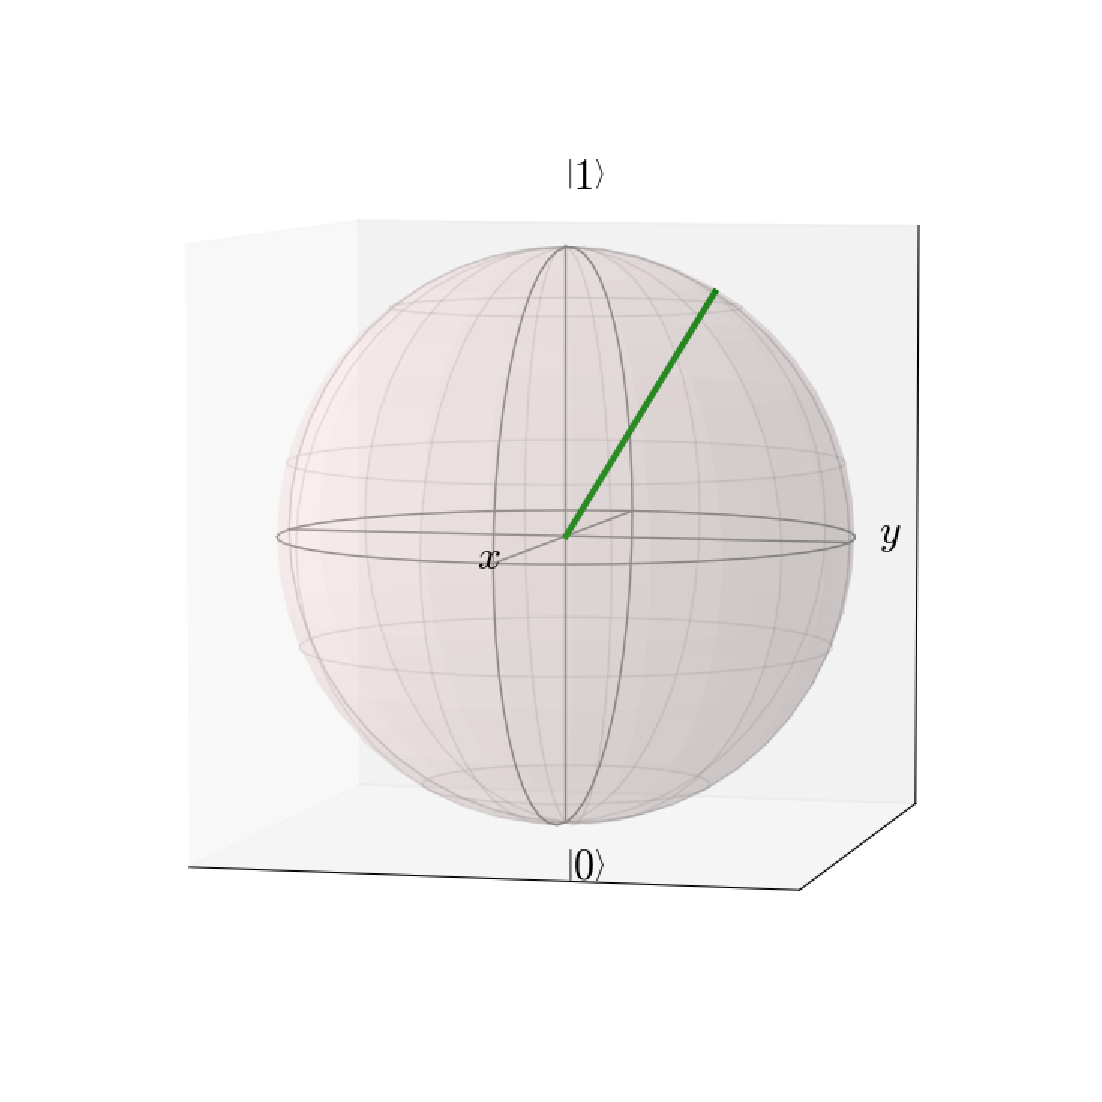
\includegraphics[width=.80\textwidth]{images/bloh1.eps} \\ а)}
\end{minipage}
\hfill
\begin{minipage}[h]{0.49\linewidth}
\center{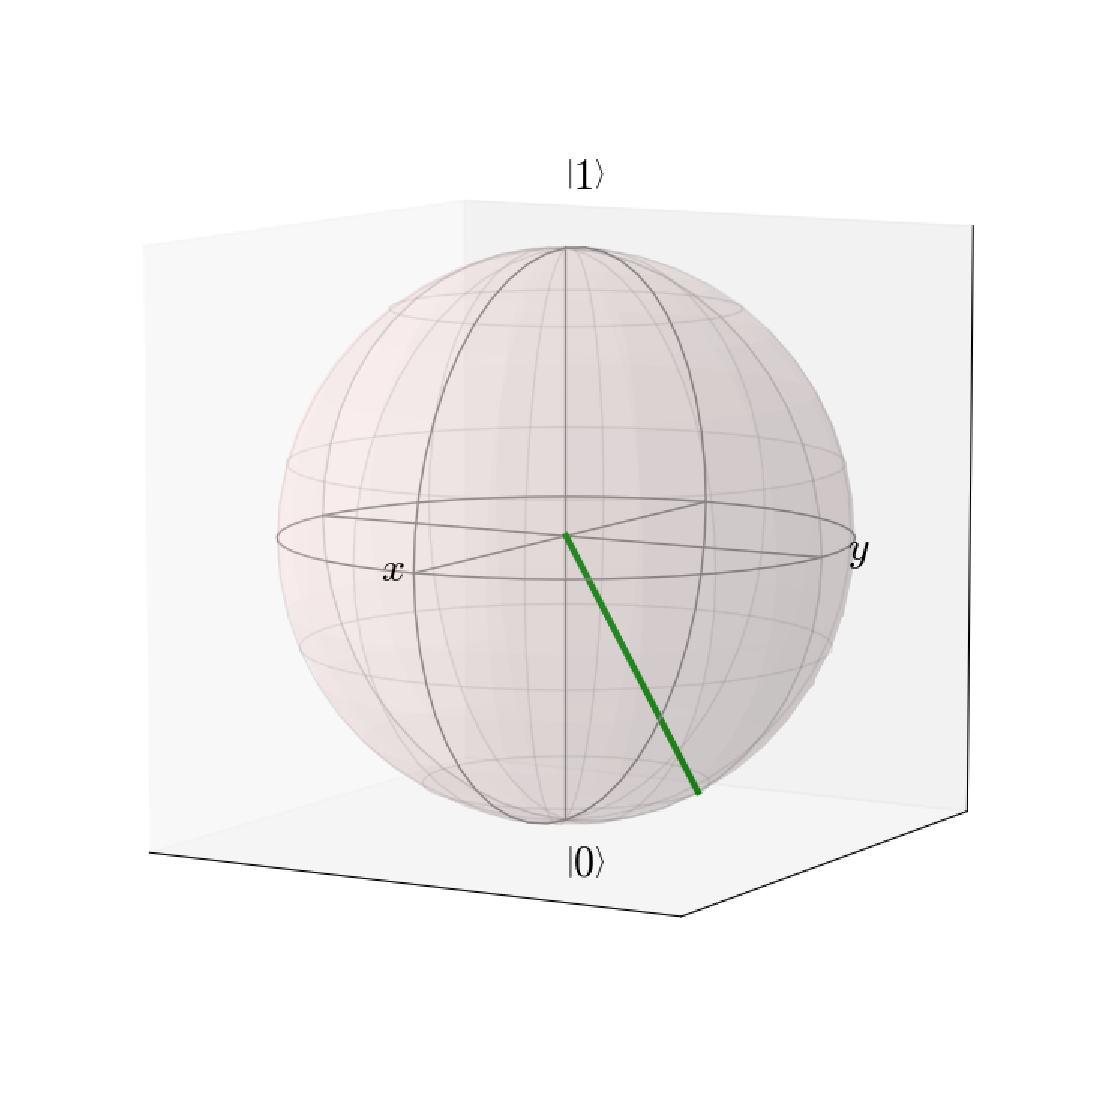
\includegraphics[width=.80\textwidth]{images/bloh2.eps} \\ б)}
\end{minipage}
\caption{Состояния (\ref{plus-position}) и (\ref{minus-position}) изображеные на сфере Блоха}
\label{ris:image1}
\end{figure}

Решения для уравнения гармонического осциллятора представлены на рисунке \ref{ris:kk1}.
\begin{figure}[h]
\centering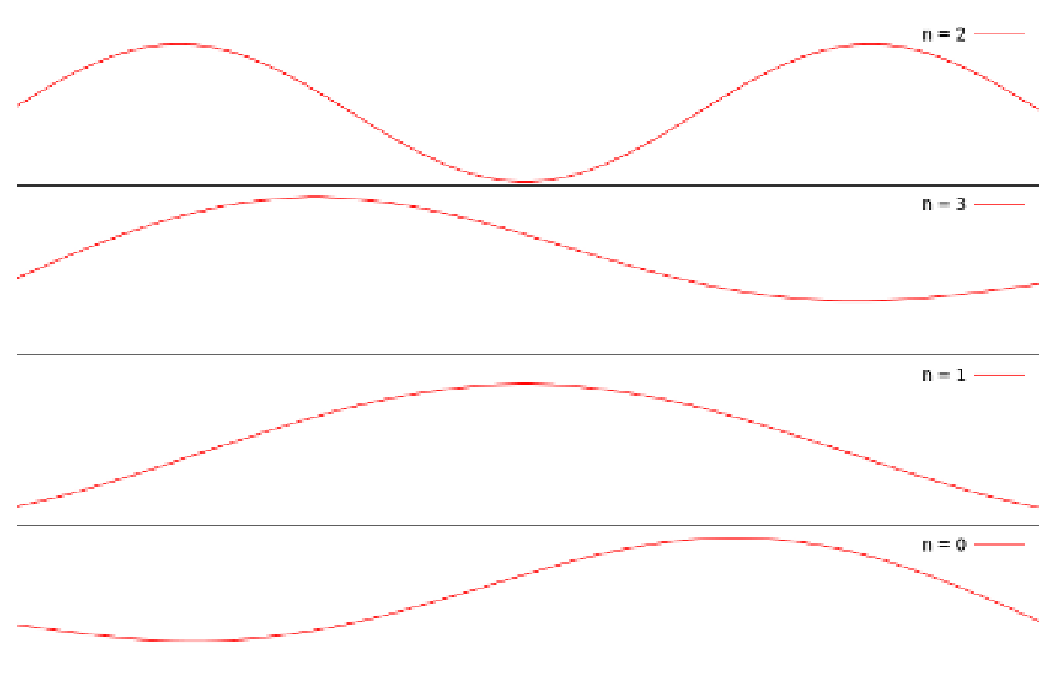
\includegraphics[width=.50\textwidth]{images/function.eps}
\caption{Собственные функции гармонического осциллятора}\label{ris:kk1}
\end{figure}

В общем случае необходимым и достаточным условием того, что с помощью данной физической системы можно реализовать унитарный оператор $U$, является
приближенное равенство собственных значений оператора $U$ и оператора эволюции $T = \exp(-iHt)$ \cite{Menskiy:2001ru}.

\section{Реализация однокубитных вычислений}
Для реализации вычислений запишем матрицу плотности, представленной системы
\begin{equation}
\rho = |\psi\rangle\langle\psi^{*}| = \begin{pmatrix} \psi_{n}\\
 						\psi_{m}
 		\end{pmatrix} \begin{pmatrix}\psi^{*}_{n} & \psi^{*}_{m}\end{pmatrix}  = \begin{pmatrix} \psi_{n}\psi^{*}_{n} & \psi_{n}\psi^{*}_{m} \\ 
 																	 					\psi_{m}\psi^{*}_{n} & \psi_{m}\psi^{*}_{m} 		 																		 
 		 																		 \end{pmatrix}
\end{equation}

Матрицу плотности можно рассматривать как оператор (оператор плотности). Если умножить её слева на произвольный вектор-столбец, то вектор-строка $\langle\psi\rvert$ умножится на него, дав скалярное произведение, а последующий за ним вектор-столбец $\lvert\psi\rangle$ умножится на это скалярное произведение, как на численный коэффициент. Итого, произвольный вектор-столбец будет рассмотрен в проекции на ось, и потом заменён на вектор вдоль этой оси, длина которого определяется проекцией. То есть, оператор --- это ровно проектор на направление, заданное исходным вектором состояния $\lvert\psi\rangle.$

Кубит может быть преобразован при помощи квантовых логических гейтов, которые осуществляются при помощи унитарного преобразования $U$, которое преобразует исходное состояние $\psi_{i}$ в состояние $\psi_{f}$ в соответствии с формулой
\begin{equation}
|\psi_{f}\rangle = U|\psi_{i}\rangle.
\end{equation}

Квантовый элемент $\mathrm{NOT}$ можно представить в матричном виде. Определим матрицу $X$ для представления квантового элемента $\mathrm{NOT}$
\begin{equation}
X \equiv \begin{bmatrix} 0 & 1 \\ 1 & 0 \end{bmatrix}.
\end{equation}
$X$ гейт действует на данный кубит следующим образом
\begin{equation}
\begin{bmatrix} 0 & 1 \\ 1 & 0 \end{bmatrix} \begin{bmatrix} \psi_{n} \\ \psi_{m} \end{bmatrix} = \begin{bmatrix} \psi_{m} \\ \psi_{n} \end{bmatrix}
\end{equation}
Квантовые элементы на одном кубите могут быть записаны матрицами размера $2 \times 2$. Матрица $U$, описывающая квантовый элемент должна быть унитарна, т.е. $U^{+}U = I$, где $U^{+}$ --- сопряжённая матрица, получаемая транспонированием и последующим комплексным сопряжением $U$, а $I$--- единичная матрица. 

Условие унитарности является единственным ограничением на квантовые элементы. Любая унитарная матрица описывает физически возможный квантовый элемент. 


\section{Спин кубита}

Частица со спином равным $1/2$ хорошо подходит для реализации кубитов. Кубит может быть образован из спиновых состояниях
одного электрона, одного ядра, пары электронов или электронно-дырочной системы (экситонов). Для электрона $z$ компонента спина равна $\pm \hbar/2$. Оператор $z$ спина 
\begin{equation}
s_{z} = \frac{\hbar}{2}\sigma_{z} \label{sh},
\end{equation}
где $\sigma_{z}$ матрица Паули
\begin{equation}
\sigma_{z} = \begin{pmatrix} 1 & 0 \\
 							 0 & -1
 			 \end{pmatrix}.
\end{equation}
Соответствующие уравнения имеют собственные формы
\begin{equation}
s_{z}|0\rangle = +\frac{\hbar}{2},   s_{z}|1\rangle = -\frac{\hbar}{2} \label{spin}.
\end{equation}
Собственные значения могут так же записанны в виде спиноров
\begin{equation}
|0\rangle = \begin{pmatrix} 1 \\
 						    0
 			 \end{pmatrix},        |1\rangle = \begin{pmatrix} 0 \\
 			    			                                   1
 			                                   \end{pmatrix}
\end{equation}
Спиновый магнитный диполь задан формулой
\begin{equation}
\mu_{z} = -\frac{1}{2}g^{*}\mu_{B}\sigma_{z},
\end{equation}
где $\mu_{B}$ магнетон Бора $(\mu_{B} = 0.927 \times 10^{-23} Am^{2})$, $g^{*}$ является эффективным фактором Ланде, который в полупроводниковых материалах может принимать как положительные, так и отрицательные значения.
Например, для электрона в $Si$ $g^{*} = 1.998$, в $Ge$ $g^{*} = 1.563$, в $GaAs$ $g^{*} = -0.44$, для электрона в ваккууме $g^{*} = 2.0$.

Спин может быть определён с помощью взаимодействия спинов магнитных диполей с внешнем магнитным полем $\vec{B}$. Для магнитного поля вида $\vec{B} = (0, 0, \vec{B})$ гамильтониан взаимодействия будет иметь вид
\begin{equation}
H_{int} = -\mu_{z}B = \frac{1}{2}g^{*}\mu_{B}\sigma_{z}B \label{gamil_vz}.
\end{equation}
Если квантовая система обладает энергией $E_{\nu}$ в отсутствии внешнего магнитного поля, тогда согластно (\ref{sh}),  (\ref{spin}) и (\ref{gamil_vz}) взаимодействие спинового магнитного диполя с магнитным полем приводит к расщеплению этого уровня энергии на два подуровня энергии
\begin{equation}
E_{\nu\pm} = E_{\nu} \pm \frac{1}{2}g^{*}\mu_{B}B \label{zeeman},
\end{equation}
где знак <<$+$>> соответствует состоянию $|0\rangle$ со спином $\hbar/2$, а знак <<$-$>> соответствует состоянию $|1\rangle$ со спином 
$-\hbar/2$. Уравнение (\ref{zeeman}) описывает спиновый эффект Зеемана \cite{Janusz:2005}. 


Чтобы выполнять произвольные квантовые вычисления, нужно иметь возможность реализовывать произвольный унитарный оператор. Например, манипулируя
параметрами $P_{x}$ и $P_{y}$, в гамильтониане $H = P_{x}X + P_{y}Y$, описывающем динамику отдельного спина, можно реализовать произвольные вращения этого спина \cite{Blum:1983ru}.

\newpage
\section{Заключение}
В ходе данной работы были получены следующие результаты:
\begin{itemize}
  \item Получено решение задачи вычисления спектра и собственных функций квантовой точки.
  \item Показано, что данная задача может быть переформулирована, как задача проведения квантовых вычислений, в которой в качестве кубита выступает электрон, помещённый в квантовую точку, а в качестве унитарного квантового оператора выступает магнитное поле.
 \end{itemize}




\newpage
\bibliographystyle{IzvAGU}
\bibliography{library}

\end{document}
